\documentclass[tikz,border=1pt]{standalone}

\usepackage{libertine}
\usetikzlibrary{arrows.meta,calc,positioning}

\definecolor{lexblue}{HTML}{DCEAF4}
\definecolor{semgreen}{HTML}{DDEEDF}
\definecolor{blindrose}{HTML}{F1DDD7}
\definecolor{stagegray}{HTML}{ECEFF1}
\definecolor{respblue}{HTML}{E4E3F2}

\begin{document}
\hyphenpenalty=10000
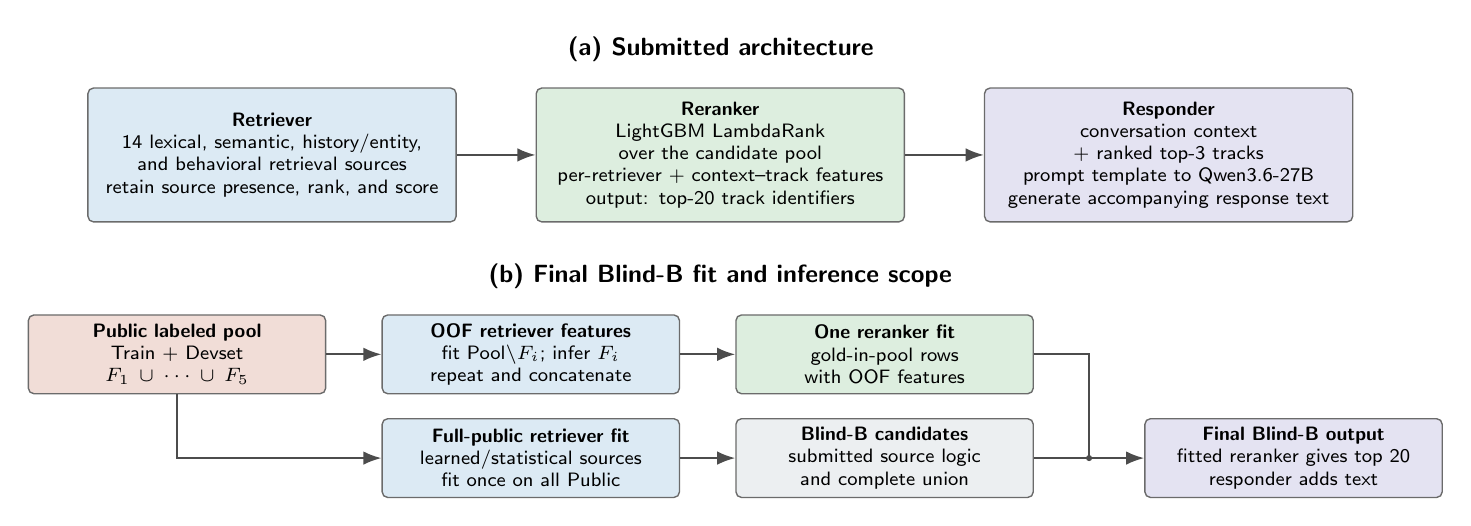
\begin{tikzpicture}[
  font=\sffamily\scriptsize,
  box/.style={draw=black!58, line width=0.5pt, rounded corners=2pt,
    align=center, minimum height=10mm, inner sep=2.5pt},
  component/.style={box, text width=45mm, minimum height=17mm},
  scope/.style={box, text width=36mm},
  flow/.style={-{Latex[length=2.3mm]}, line width=0.75pt, draw=black!70},
  mergeflow/.style={line width=0.75pt, draw=black!70},
]
  \node[font=\sffamily\small\bfseries] (architecture-title)
    {(a) Submitted architecture};
  \node[component, fill=lexblue, below=2mm of architecture-title, xshift=-57mm]
    (retriever) {\textbf{Retriever}\\14 lexical, semantic, history/entity,\\
    and behavioral retrieval sources\\retain source presence, rank, and score};
  \node[component, fill=semgreen, right=10mm of retriever] (reranker)
    {\textbf{Reranker}\\LightGBM LambdaRank over the candidate pool\\
    per-retriever + context--track features\\output: top-20 track identifiers};
  \node[component, fill=respblue, right=10mm of reranker] (responder)
    {\textbf{Responder}\\conversation context + ranked top-3 tracks\\
    prompt template to Qwen3.6-27B\\generate accompanying response text};
  \draw[flow] (retriever.east) -- (reranker.west);
  \draw[flow] (reranker.east) -- (responder.west);

  \node[font=\sffamily\small\bfseries, below=4mm of reranker]
    (scope-title) {(b) Final Blind-B fit and inference scope};
  \node[scope, fill=blindrose, below=2mm of scope-title, xshift=-69mm]
    (public-pool) {\textbf{Public labeled pool}\\Train + Devset\\
    $F_1\cup\cdots\cup F_5$};
  \node[scope, fill=lexblue, right=7mm of public-pool] (public-oof)
    {\textbf{OOF retriever features}\\fit Pool$\setminus F_i$; infer $F_i$\\
    repeat and concatenate};
  \node[scope, fill=semgreen, right=7mm of public-oof] (public-ranker)
    {\textbf{One reranker fit}\\gold-in-pool rows\\with OOF features};
  \node[scope, fill=lexblue, below=3mm of public-oof] (full-retriever)
    {\textbf{Full-public retriever fit}\\learned/statistical sources\\fit once on all Public};
  \node[scope, fill=stagegray, below=3mm of public-ranker] (blind-candidates)
    {\textbf{Blind-B candidates}\\submitted source logic\\and complete union};
  \node[scope, fill=respblue, right=14mm of blind-candidates]
    (blind-target) {\textbf{Final Blind-B output}\\fitted reranker gives top 20\\
    responder adds text};
  \draw[flow] (public-pool.east) -- (public-oof.west);
  \draw[flow] (public-oof.east) -- (public-ranker.west);
  \draw[flow] (public-pool.south) |- (full-retriever.west);
  \draw[flow] (full-retriever.east) -- (blind-candidates.west);
  \coordinate (blind-merge) at ($(blind-candidates.east)!0.5!(blind-target.west)$);
  \draw[mergeflow] (public-ranker.east) -| (blind-merge);
  \draw[mergeflow] (blind-candidates.east) -- (blind-merge);
  \fill[black!70] (blind-merge) circle (1.1pt);
  \draw[flow] (blind-merge) -- (blind-target.west);
\end{tikzpicture}
\end{document}
